\documentclass[11pt,letterpaper]{article}

\usepackage[spanish,es-nodecimaldot]{babel}
\usepackage[utf8]{inputenc}
\usepackage[T1]{fontenc}
\usepackage{lmodern}
\usepackage{geometry}
\usepackage{graphicx}
\usepackage{xcolor}
\usepackage{tikz}
\usepackage[most]{tcolorbox}
\usepackage{tabularx}
\usepackage{booktabs}
\usepackage{array}
\usepackage{longtable}
\usepackage{enumitem}
\usepackage{titlesec}
\usepackage{fancyhdr}
\usepackage{lastpage}
\usepackage{caption}
\usepackage{float}
\usepackage{hyperref}
\usepackage{microtype}

\usetikzlibrary{arrows.meta,positioning,calc,shadows.blur}

\geometry{margin=2.5cm}


\definecolor{paper}{HTML}{F4F1E8}
\definecolor{ink}{HTML}{17211D}
\definecolor{muted}{HTML}{5C6A65}
\definecolor{deepgreen}{HTML}{0B1F1B}
\definecolor{pine}{HTML}{173C32}
\definecolor{moss}{HTML}{2D5A43}
\definecolor{fog}{HTML}{C7D1CF}
\definecolor{rail}{HTML}{D7DEE0}
\definecolor{railshadow}{HTML}{8D9699}
\definecolor{trackbed}{HTML}{6B5747}
\definecolor{wood}{HTML}{7B5A3B}
\definecolor{amber}{HTML}{F7C66A}
\definecolor{rust}{HTML}{A65D3D}
\definecolor{danger}{HTML}{A83A2D}
\definecolor{night}{HTML}{111827}

\hypersetup{
  colorlinks=true,
  linkcolor=pine,
  urlcolor=rust,
  citecolor=pine,
  pdftitle={Informe de Entorno Virtual - Echoes of the Rails},
  pdfauthor={Grupo N°1}
}

\setlength{\parindent}{0pt}
\setlength{\parskip}{0.52em}
\setlength{\headheight}{22pt}
\renewcommand{\arraystretch}{1.25}
\setlist[itemize]{leftmargin=1.35em,itemsep=0.18em,topsep=0.25em}
\setlist[enumerate]{leftmargin=1.5em,itemsep=0.22em,topsep=0.25em}

\titleformat{\section}
  {\normalfont\Large\bfseries\color{deepgreen}}
  {\thesection}{0.75em}{}
\titleformat{\subsection}
  {\normalfont\large\bfseries\color{pine}}
  {\thesubsection}{0.65em}{}
\titleformat{\subsubsection}
  {\normalfont\normalsize\bfseries\color{rust}}
  {\thesubsubsection}{0.55em}{}

\captionsetup{
  labelfont={bf,color=pine},
  textfont={small,color=muted},
  font=small
}

\pagestyle{fancy}
\fancyhf{}
\lhead{\sffamily\small Echoes of the Rails}
\rhead{\sffamily\small Entorno virtual}
\cfoot{\sffamily\small \thepage\ de \pageref{LastPage}}
\renewcommand{\headrulewidth}{0.4pt}
\renewcommand{\headrule}{\hbox to\headwidth{\color{fog}\leaders\hrule height \headrulewidth\hfill}}

\newcolumntype{Y}{>{\raggedright\arraybackslash}X}
\newcolumntype{L}[1]{>{\raggedright\arraybackslash}p{#1}}
\newcolumntype{C}[1]{>{\centering\arraybackslash}p{#1}}

\newtcolorbox{infoCard}[1][]{
  enhanced,
  breakable,
  colback=white,
  colframe=fog,
  boxrule=0.6pt,
  arc=2.5mm,
  left=3.5mm,right=3.5mm,top=3mm,bottom=3mm,
  borderline west={2pt}{0pt}{pine},
  #1
}

\begin{document}

\begin{titlepage}
\thispagestyle{empty}
\begin{tikzpicture}[remember picture,overlay]
  \fill[white] (current page.south west) rectangle (current page.north east);
  \fill[deepgreen] (current page.north west) rectangle ([xshift=3.6cm]current page.south west);
  \fill[pine] ([xshift=3.05cm]current page.north west) -- ([xshift=4.35cm]current page.north west) -- ([xshift=3.45cm]current page.south west) -- ([xshift=2.25cm]current page.south west) -- cycle;
  \draw[amber,line width=1pt] ([xshift=11.8cm,yshift=-1.05cm]current page.north west) -- ([xshift=-1.1cm,yshift=-1.05cm]current page.north east);
  \draw[amber,line width=1pt] ([xshift=4.5cm,yshift=1.05cm]current page.south west) -- ([xshift=-1.1cm,yshift=1.05cm]current page.south east);
\end{tikzpicture}

\vspace*{1.8cm}
\hspace*{4.15cm}
\begin{minipage}{0.68\textwidth}
\begin{flushleft}
{\Large\bfseries Universidad de las Fuerzas Armadas ESPE\par}
\vspace{0.2cm}
{\large Desarrollo de Videojuegos -- 30817\par}
\vspace{2.0cm}
{\fontsize{25}{31}\selectfont\bfseries Echoes of the Rails\par}
\vspace{0.3cm}
{\Large Informe de diseño del entorno virtual\par}
\vspace{1.6cm}
\begin{tikzpicture}
\draw[amber,line width=1pt] (0,0) -- (9.4,0);
\fill[amber] (0,0) circle (2pt);
\fill[amber] (9.4,0) circle (2pt);
\end{tikzpicture}
\vspace{0.65cm}

{\bfseries Tarea I -- Parcial I\par}
\vspace{0.3cm}
{\bfseries Docente:} Ing. Héctor Pinto\par
\vspace{0.3cm}
{\bfseries Grupo N\textsuperscript{o}1:} Jordan Guaman, Mesías Mariscal, Anthony Morales, Denise Rea\par
\vspace{0.3cm}
{\bfseries Carrera:} Ingeniería en Software\par
\vspace{1.0cm}
Sangolquí, Ecuador\par
Mayo de 2026
\end{flushleft}
\end{minipage}
\end{titlepage}

\tableofcontents
\newpage

\section{Coherencia del Entorno con el Videojuego}

El entorno de \textit{Echoes of the Rails} está diseñado para responder a los pilares del videojuego: objetivo medible, historia, género y mecánicas. La ruta se define como un sistema funcional de toma de decisiones: avanzar, administrar carbón, cumplir tiempos de llegada y evitar pérdida de pasajeros en condiciones de niebla.

\subsection{Coherencia con el Objetivo del Juego}

\begin{infoCard}
\textbf{Objetivo principal:} completar al menos 5 rutas consecutivas sin que el carbón llegue a cero y llegar a un mínimo del 60\% de las estaciones activas.
\end{infoCard}

El escenario responde directamente a este objetivo porque:

\begin{itemize}
  \item El sistema de vías sobre ruta continua permite encadenar recorridos sin interrupciones.
  \item Las estaciones distribuidas por el trayecto convierten el avance en metas parciales.
  \item La niebla limita la visibilidad y vuelve más tensa la lectura del siguiente tramo.
  \item La cabina y sus medidores recuerdan constantemente el consumo de carbón y la velocidad.
  \item Las pendientes, curvas y rectas obligan a equilibrar rapidez con seguridad.
\end{itemize}

\begin{figure}[H]
\centering
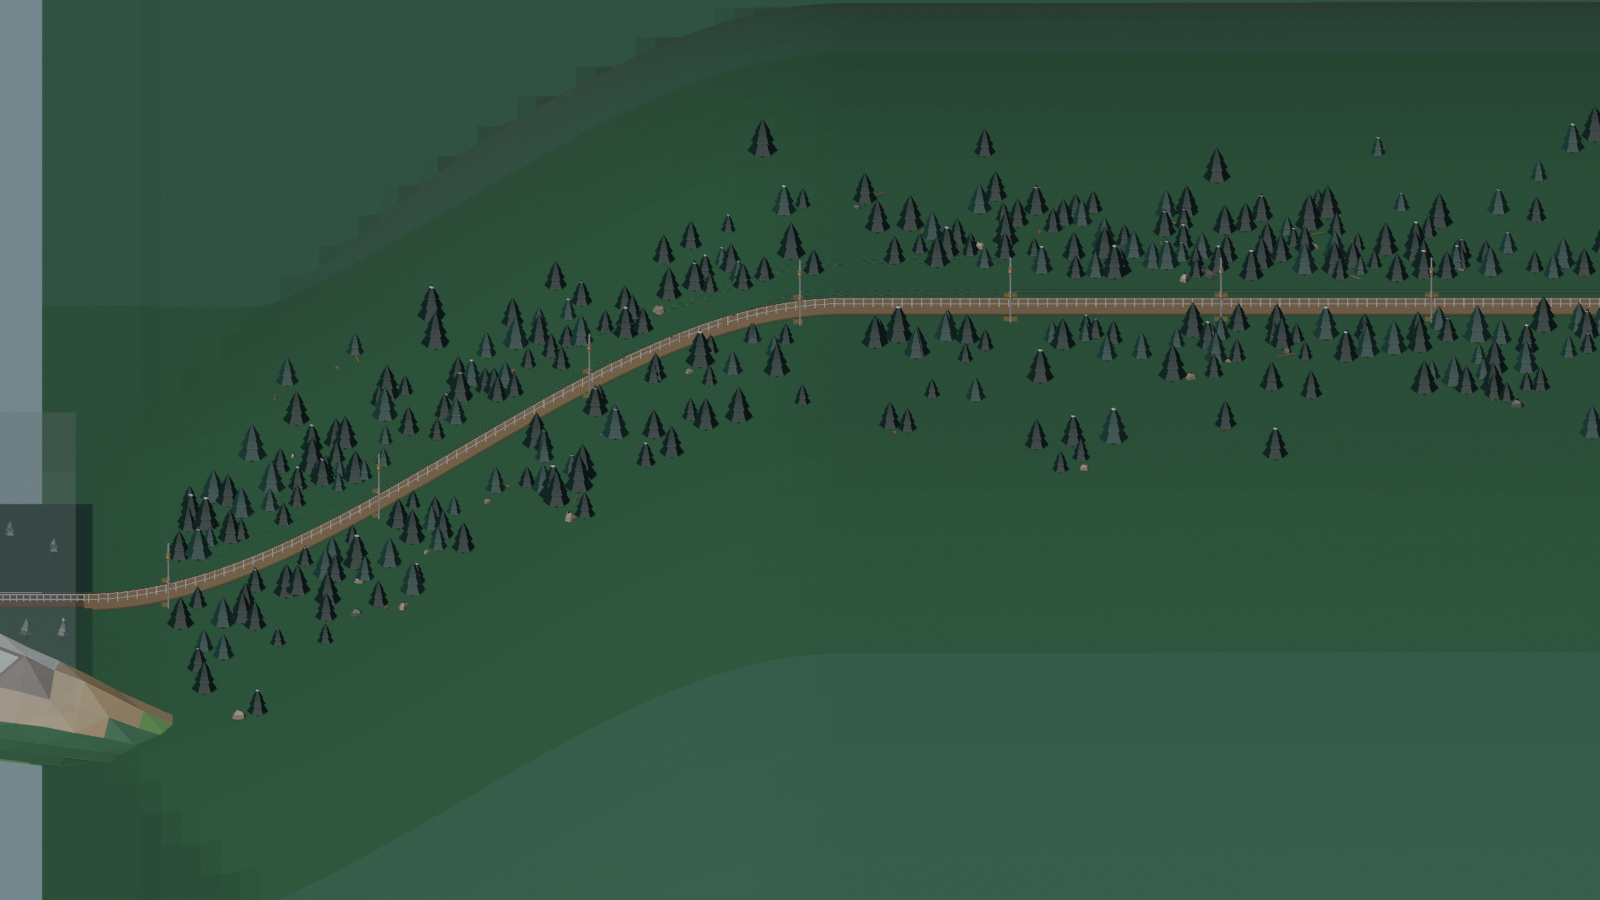
\includegraphics[width=\textwidth]{figures/blender_actual_recorrido_general.png}
\caption{Vista actual del escenario en Blender: ruta ferroviaria de montaña con bosque, ascenso, cima, estaciones y postes junto a la vía.}
\end{figure}

\begin{figure}[H]
\centering
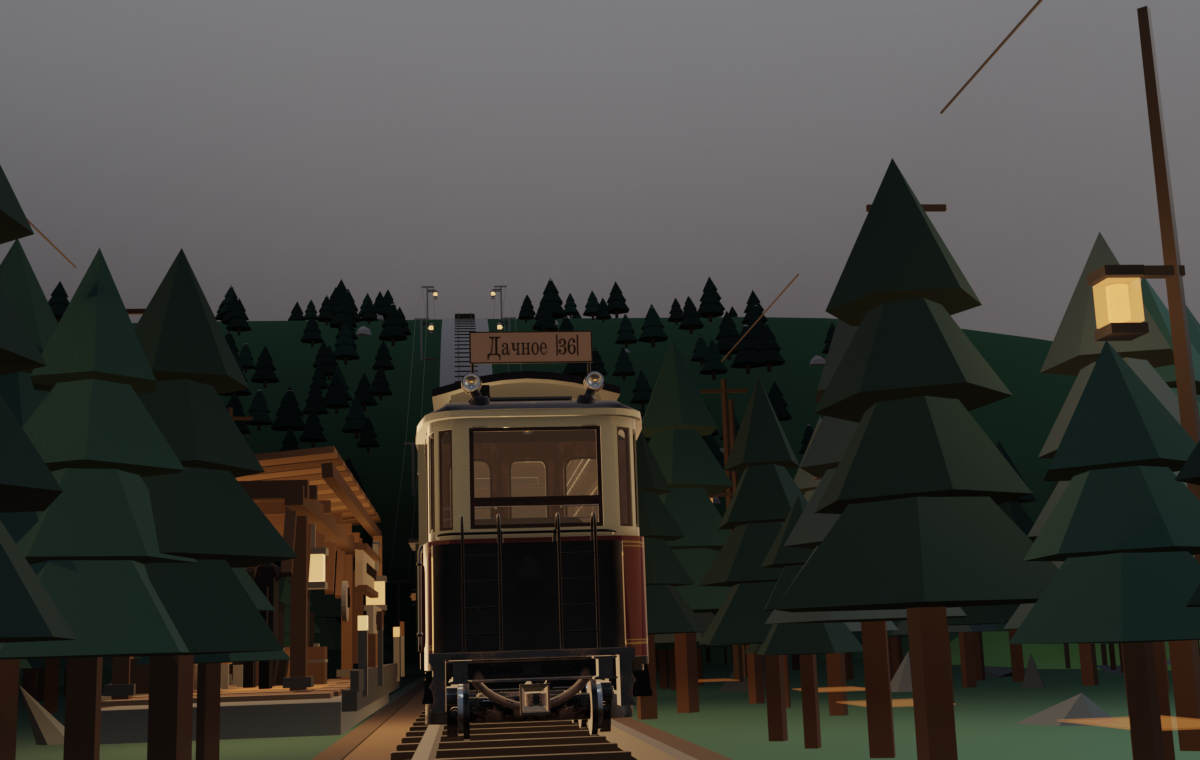
\includegraphics[width=\textwidth]{figures/figura2_vista.png}
\caption{Vista complementaria del entorno con lectura funcional del recorrido y su integración visual en la ruta principal.}
\end{figure}

\subsection{Coherencia con la Historia}

La narrativa presenta al jugador como el último maquinista de una línea ferroviaria olvidada en una zona montañosa sin acceso por carretera. El entorno materializa esta idea mediante una estática de aislamiento: montañas extensas, pinos alrededor de la vía, estaciones pequeñas, farolas cálidas y niebla persistente.

La ausencia de una interfaz externa mantiene la coherencia diegética de la simulación. El jugador observa la ruta desde la cabina y depende de los instrumentos, las señales visuales y los puntos de luz para orientarse. Las estaciones no son solo puntos de parada: son momentos narrativos donde los pasajeros esperan, abordan o desaparecen cuando el tren llega tarde.

\subsection{Coherencia con el Género y las Mecánicas}

\begin{table}[H]
\centering
\begin{tabularx}{\textwidth}{@{}L{4cm}Y@{}}
\toprule
\textbf{Campo} & \textbf{Detalle}\\
\midrule
Género & Simulación ferroviaria VR / Gestión de recursos / Horror sutil\\
Plataforma objetivo & Godot 4.6 + OpenXR\\
Mecánica central & Equilibrio entre velocidad, consumo de carbón y presión temporal\\
Estilo visual & Retro Realism con estática low-poly y atmósfera de niebla\\
\bottomrule
\end{tabularx}
\caption{Relación general entre el entorno y el género del videojuego.}
\end{table}

La simulación requiere un espacio legible con niveles de riesgo controlado. Por eso el entorno combina rieles claros, estaciones reconocibles, postes con farolas y una montaña que altera la lectura del recorrido. La gestión de recursos se justifica con el ascenso, la distancia entre estaciones y la necesidad de frenar antes de curvas o paradas.

\section{Diseño Visual y Ambientación del Escenario}

El escenario de \textit{El Paso de la Bruma} trabaja una identidad visual \textit{Retro Realism}: modelos de baja poligonización, materiales de lectura clara, colores contenidos, luces cálidas puntuales y niebla atmosférica. Para describir la paleta se toma como referencia la vista con materiales activos en Blender, no el modo \textit{Solid}, porque este último puede mostrar modelos complejos en blanco o con colores planos que no representan el acabado final.

\subsection{Paleta de Color e Iluminación}

\begin{table}[H]
\centering
\begin{tabularx}{\textwidth}{@{}L{4cm}L{3.4cm}Y@{}}
\toprule
\textbf{Elemento} & \textbf{Color guía} & \textbf{Función visual}\\
\midrule
Cielo nocturno & Azul oscuro & Crea soledad y calma tensa.\\
Neblina de ruta & Gris niebla & Reduce visibilidad y separa planos de profundidad.\\
Madera y tierra & Marrón cálido & Conecta vías, estación, andenes y desgaste ferroviario.\\
Locomotora y vagón & Rojo oscuro, crema, negro y metal envejecido & Diferencia el vehículo principal del terreno y comunica uso, antigüedad y peso.\\
Rieles metálicos & Gris claro & Hace legible el recorrido del tren.\\
Vegetación & Verde oscuro & Rodea la vía y refuerza el aislamiento de montaña.\\
Iluminación de andén & Amarillo tenue & Marca puntos humanos dentro del bosque.\\
\bottomrule
\end{tabularx}
\caption{Paleta visual aplicada al entorno.}
\end{table}

La iluminación se mantiene tenue para que las farolas, la estación y la cabina tengan protagonismo. En el recorrido de Blender, las farolas acompañan los postes y ayudan a leer los bordes de la vía sin invadir el espacio central de circulación. La locomotora importada conserva texturas de color, rugosidad metálica y normales; por ello su lectura real corresponde al acabado desgastado visible en vista de materiales.

\begin{figure}[H]
\centering
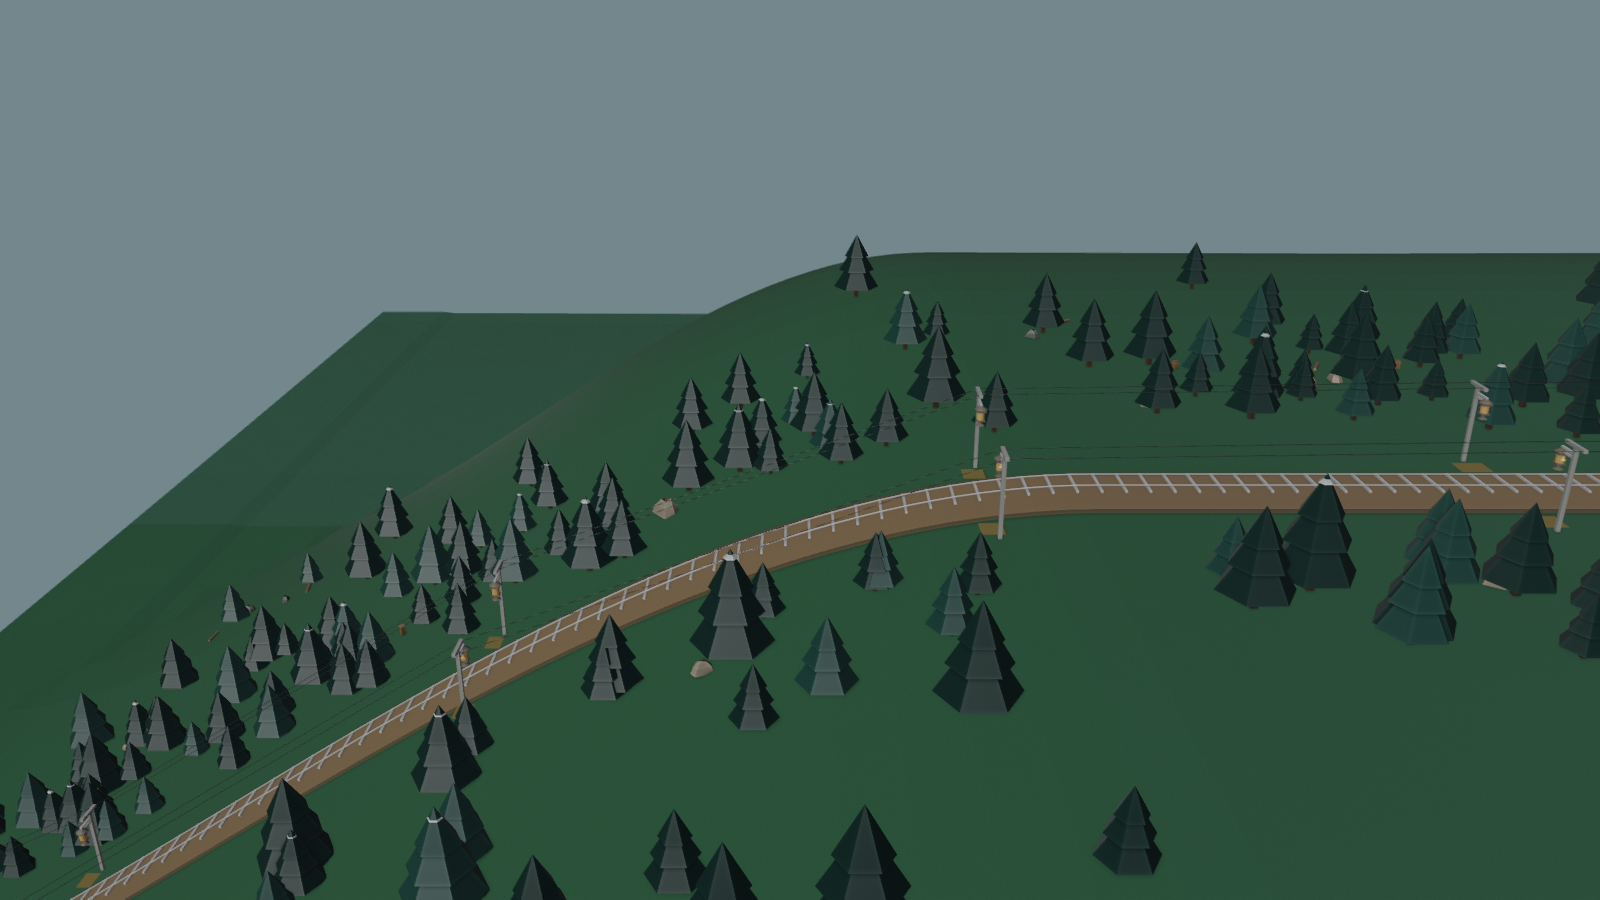
\includegraphics[width=0.96\textwidth]{figures/blender_actual_estacion_cima.png}
\caption{Composición actual de la cima: rieles, árboles, postes y farolas organizados alrededor del corredor ferroviario.}
\end{figure}

\subsection{Composición y Uso del Espacio}

La composición del escenario se organiza en tres capas:

\begin{itemize}
  \item \textbf{Primer plano:} locomotora, vagón posterior y cabina VR, donde el jugador toma decisiones.
  \item \textbf{Plano medio:} rieles, tierra de vía, estación, postes, farolas y puntos de parada.
  \item \textbf{Fondo:} montaña, bosque, rocas y niebla que dan profundidad sin sobrecargar la escena.
\end{itemize}

El diseño evita que los árboles aparezcan en medio de los rieles. La vegetación se concentra alrededor de la vía para crear un corredor visual, mientras que la tierra y los rieles permanecen despejados para que el jugador anticipe curvas, ascensos y estaciones.

\begin{figure}[H]
\centering
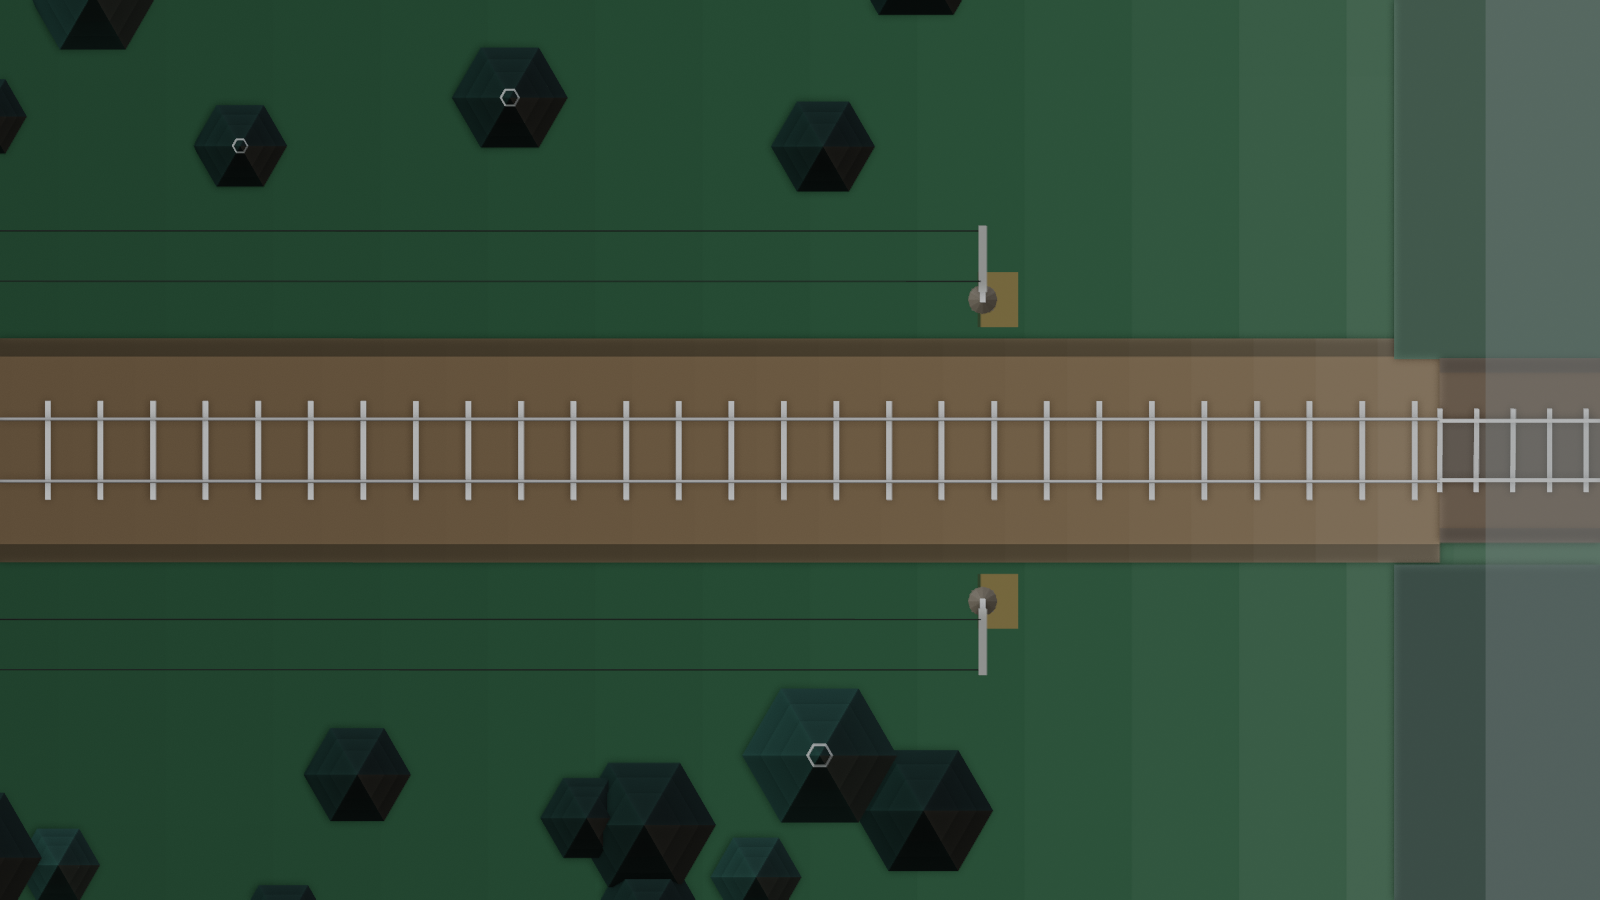
\includegraphics[width=0.96\textwidth]{figures/blender_actual_ancho_montana.png}
\caption{Vista superior del ancho del terreno y del corredor de rieles, con árboles y rocas ubicados fuera del paso del tren.}
\end{figure}

\subsection{Estilo Visual Retro Realism}

La baja poligonización no se plantea como limitación, sino como decisión artística. Los árboles, rocas, montaña y estaciones usan formas simples que recuerdan videojuegos de los años noventa. Esta decisión también es funcional: reduce carga visual, mantiene legibilidad en VR y permite usar niebla sin afectar demasiado el rendimiento.

\section{Elementos y Objetos del Entorno}

El entorno se sostiene sobre objetos principales, decorativos e interactivos. Esta separación ayuda a explicar qué elementos estructuran la jugabilidad y cuáles aportan ambientación.

\subsection{Objetos Principales}

\begin{longtable}{@{}L{4.2cm}L{11.2cm}@{}}
\toprule
\textbf{Objeto principal} & \textbf{Función en el entorno}\\
\midrule
\endfirsthead
\toprule
\textbf{Objeto principal} & \textbf{Función en el entorno}\\
\midrule
\endhead
Locomotora y vagón posterior & Vehículo del jugador y silueta central del juego. La locomotora frontal importada desde Sketchfab se conecta con el vagón mediante una cadena, evitando que el tren parezca un ?nico vagón aislado.\\
Vías ferroviarias & Definen la ruta continua, conectan estaciones y marcan el recorrido que debe leer el jugador.\\
Montaña y colina extendida & Generan ascenso, cima y descenso, haciendo que la ruta tenga ritmo y tensión.\\
Andenes / estaciones & Funcionan como objetivos temporales donde se resuelve si el jugador llega a tiempo.\\
Cabina de control & Integra tablero, palancas, freno, medidores y decisiones principales en VR.\\
\bottomrule
\caption{Objetos principales que sostienen la experiencia jugable.}
\end{longtable}

\begin{figure}[H]
\centering
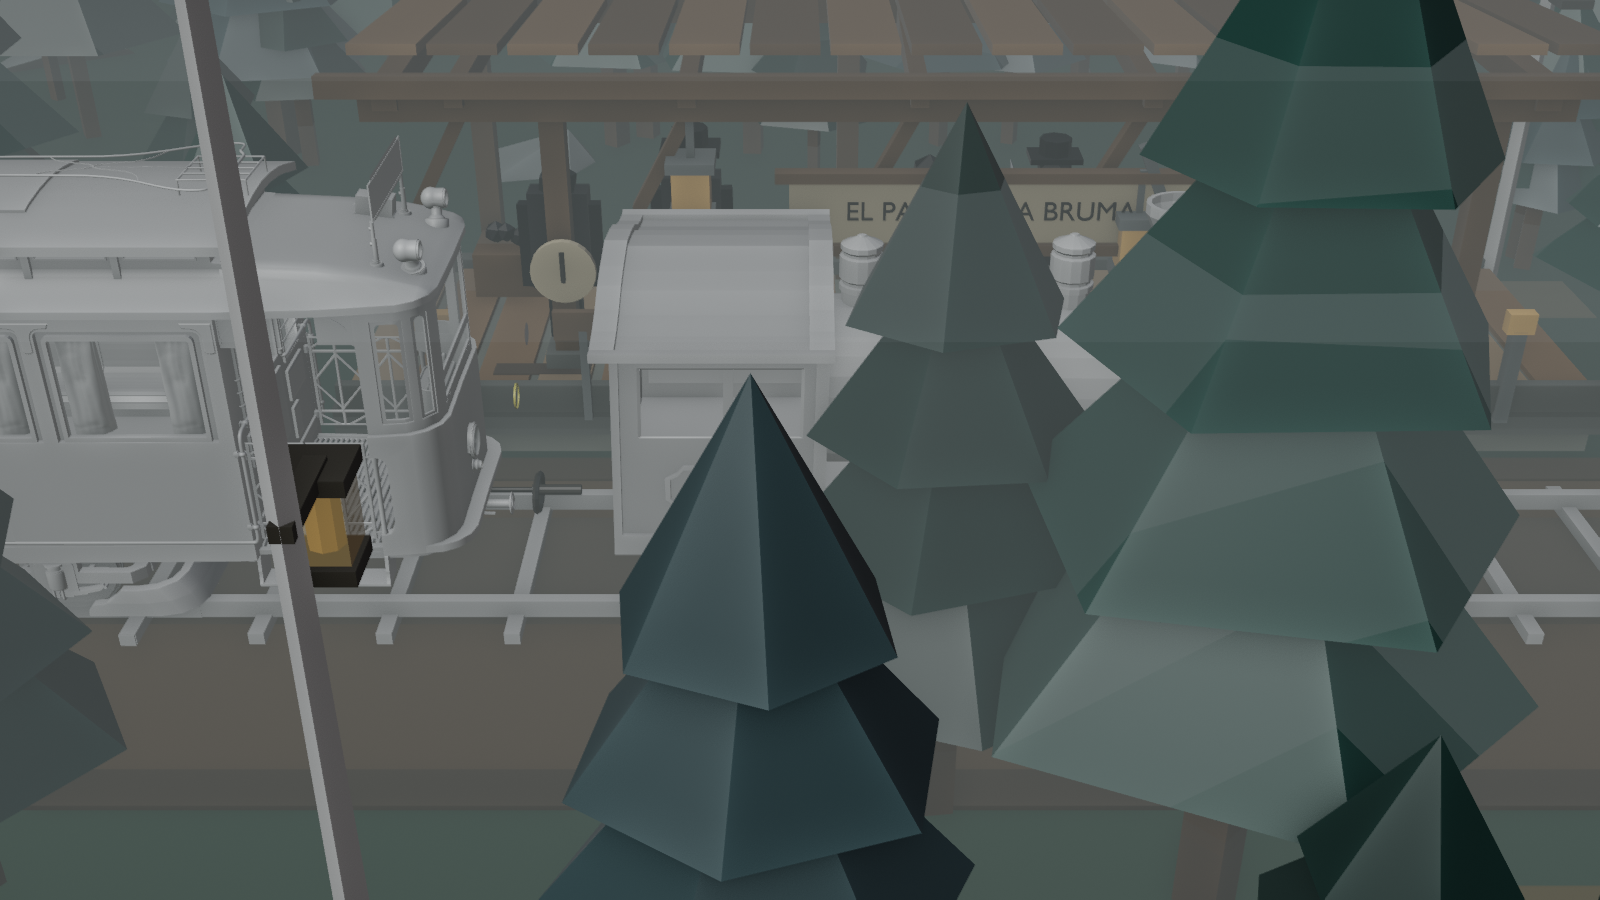
\includegraphics[width=0.92\textwidth]{figures/blender_actual_locomotora_vagones.png}
\caption{Locomotora y vagón posterior dentro del entorno actual, integrados con estación, árboles, postes y niebla.}
\end{figure}

\subsection{Objetos Decorativos}

\begin{longtable}{@{}L{4.2cm}L{11.2cm}@{}}
\toprule
\textbf{Objeto decorativo} & \textbf{Aporte al ambiente}\\
\midrule
\endfirsthead
\toprule
\textbf{Objeto decorativo} & \textbf{Aporte al ambiente}\\
\midrule
\endhead
Bosque de pinos low-poly & Enmarca visualmente la ruta y refuerza el aislamiento montañoso.\\
Rocas, troncos y tocones & Rompen la uniformidad del terreno y hacen que el bosque se sienta más natural.\\
Farolas y postes & Marcan la presencia humana, guían la mirada y completan la lectura nocturna de la vía.\\
Cables ferroviarios & Aportan continuidad técnica y conectan visualmente los postes del recorrido.\\
Niebla volumétrica & Limita la visibilidad, crea profundidad y refuerza la melancolía del juego.\\
Cielo nublado perpetuo & Mantiene una iluminación difusa y una atmósfera de espera constante.\\
\bottomrule
\caption{Objetos de ambientación que construyen el tono visual.}
\end{longtable}

\begin{figure}[H]
\centering
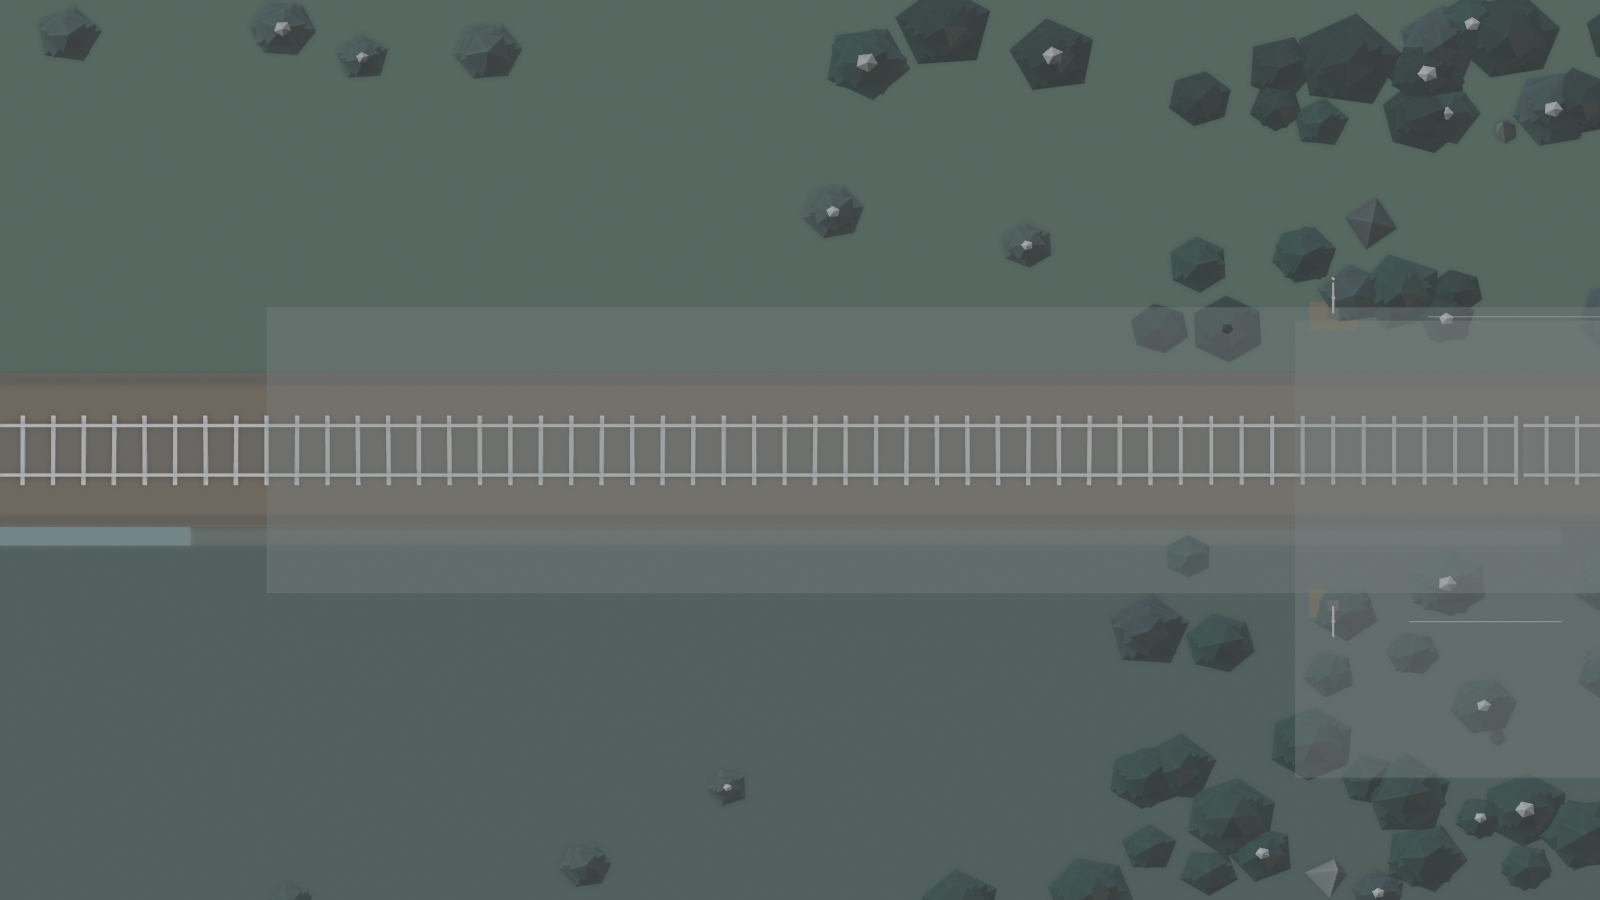
\includegraphics[width=0.96\textwidth]{figures/blender_actual_conexion_rieles.png}
\caption{Lectura superior de los rieles, la tierra de vía y los postes: el corredor central queda despejado para que la ruta sea funcional.}
\end{figure}

\subsection{Objetos Interactivos}

\begin{table}[H]
\centering
\begin{tabularx}{\textwidth}{@{}L{4.2cm}Y@{}}
\toprule
\textbf{Objeto interactivo} & \textbf{Función}\\
\midrule
Regulador de vapor & Controla la velocidad y aumenta el consumo de carbón.\\
Freno neumático & Permite detenerse con precisión en andenes y reducir velocidad en curvas.\\
Panel de suministros & Permite comprar carbón con puntos obtenidos al transportar pasajeros.\\
Temporizador de estación & Cuenta regresiva que define si los pasajeros abordan o se pierden.\\
Medidores de cabina & Muestran velocidad, carbón, presión y estado del viaje sin HUD externo.\\
\bottomrule
\end{tabularx}
\caption{Objetos interactivos ligados a la toma de decisiones del jugador.}
\end{table}

\subsection{Pasajeros NPC}

Los pasajeros funcionan como elementos híbridos entre ambiente e interacción. Visualmente aparecen como figuras silenciosas en el andén; mecánicamente representan la recompensa o pérdida del jugador.

\begin{itemize}
  \item \textbf{Esperar:} permanecen en la estación mientras el temporizador está activo.
  \item \textbf{Abordar:} suben si el tren llega a tiempo y se detiene correctamente.
  \item \textbf{Retirarse:} desaparecen en la niebla si el temporizador llega a cero.
\end{itemize}

\subsection{Notas y Memorias de Pasajeros / Almas}

Como parte del sistema narrativo del entorno, se incorpora el apartado de notas o memorias asociadas a los pasajeros (almas) que suben a la locomotora. Estas memorias funcionan como evidencia diegética del paso de cada viajero y refuerzan la relación entre la conducción del tren y la carga emocional del recorrido.

\begin{itemize}
  \item \textbf{Activación:} la memoria se habilita al completar correctamente el abordaje en estación.
  \item \textbf{Persistencia:} la nota queda vinculada al progreso de ruta y al estado del viaje.
  \item \textbf{Pérdida:} si el jugador no llega a tiempo, la memoria de ese pasajero no se registra.
\end{itemize}

\subsection{Imágenes de Memorias}

\begin{figure}[H]
\centering
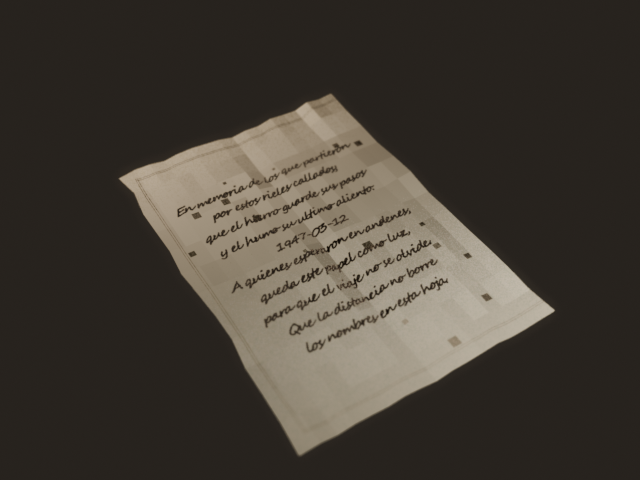
\includegraphics[width=0.72\textwidth]{figures/memoria_pasajero_nota.png}
\caption{Ejemplo de nota/memoria asociada a pasajeros que abordan la locomotora.}
\end{figure}

\section{Funcionalidad e Interacción del Entorno}

El entorno genera decisiones con consecuencias. El jugador no solo avanza por una ruta: debe interpretar pendiente, curvas, estaciones, niebla y consumo de carbón.

\subsection{Rutas y Zonas de Exploración}

\begin{table}[H]
\centering
\begin{tabularx}{\textwidth}{@{}L{3.7cm}Y Y@{}}
\toprule
\textbf{Zona} & \textbf{Descripción} & \textbf{Impacto en jugabilidad}\\
\midrule
Cabina VR & Zona principal de interacción con tablero y controles. & Concentra las decisiones del jugador y evita depender de un HUD externo.\\
Tramo recto & Segmento donde el consumo y la velocidad son predecibles. & Permite acelerar y planificar el carbón restante.\\
Curvas cerradas & Cambios de dirección donde la velocidad excesiva puede ser peligrosa. & Obliga a frenar y leer la vía con anticipación.\\
Pendientes & Ascensos y descensos de montaña. & Subir consume más; bajar exige controlar la velocidad.\\
Andenes / estaciones & Puntos de parada con pasajeros y temporizadores. & Resuelven éxito, pérdida o recompensa narrativa.\\
Zona de niebla densa & Espacio de baja visibilidad más allí del tramo inmediato. & Oculta el futuro de la ruta y aumenta la presión temporal.\\
\bottomrule
\end{tabularx}
\caption{Zonas funcionales del entorno.}
\end{table}

\begin{figure}[H]
\centering
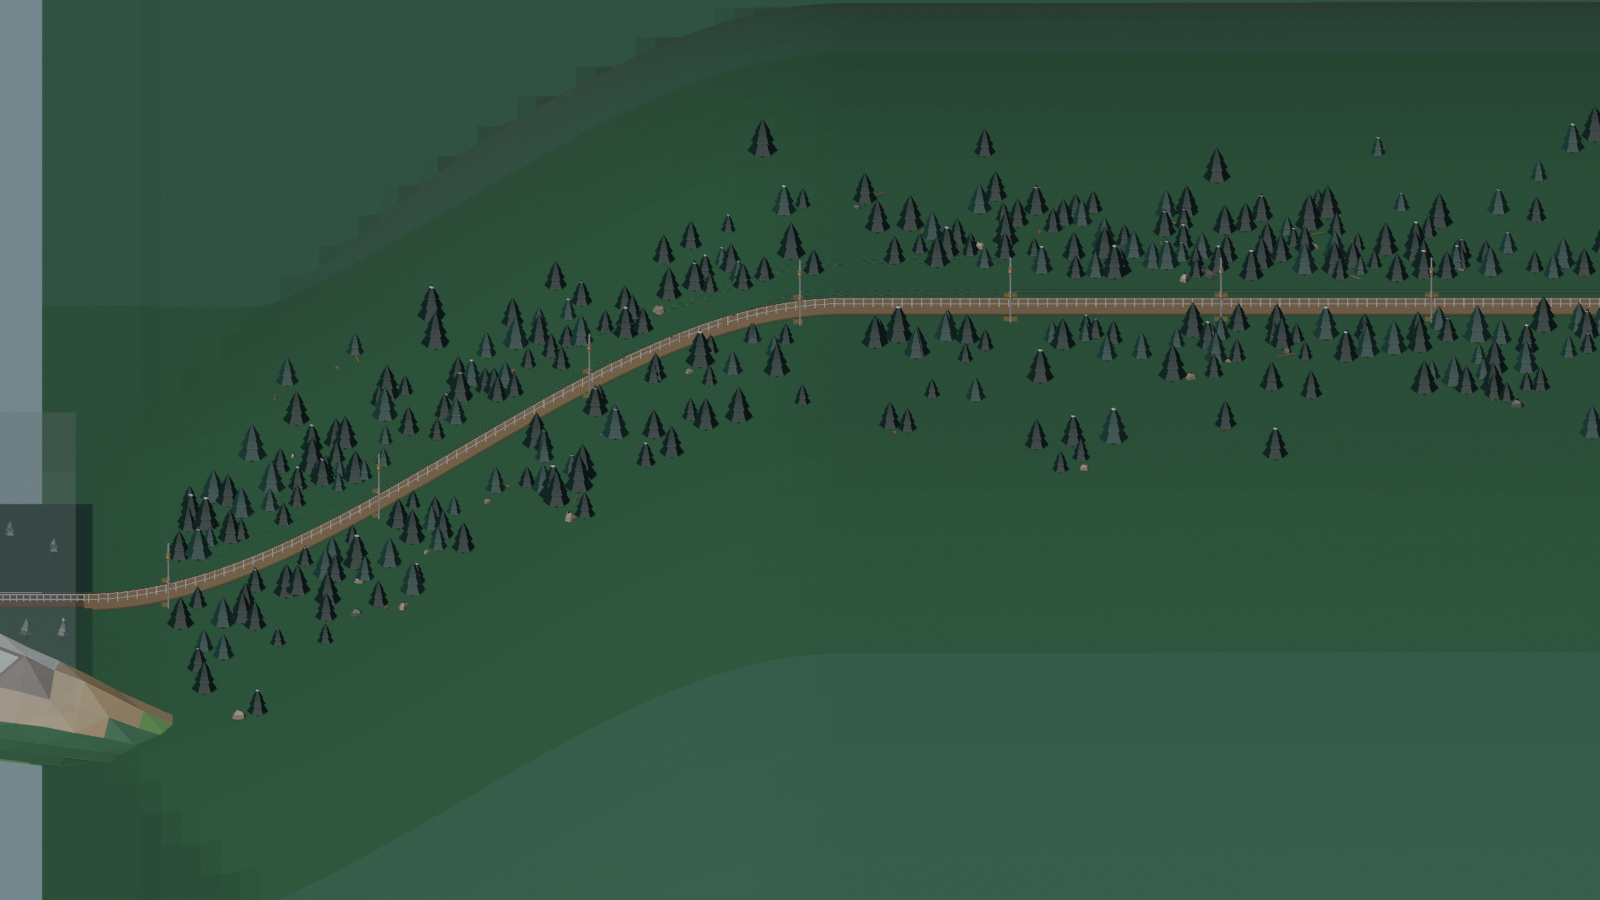
\includegraphics[width=0.96\textwidth]{figures/blender_actual_recorrido_general.png}
\caption{Recorrido completo: la ruta sube, se extiende por la cima y desciende hacia nuevas paradas sin cortar la lectura del trayecto.}
\end{figure}

La cabina interior trabajada en Godot complementa este diseño exterior. Funciona como punto de vista del maquinista y concentra instrumentos, palancas, freno y lectura de recursos; por eso el entorno no se entiende solo como paisaje, sino como el espacio que el jugador interpreta desde dentro del tren.

\subsection{Obstáculos del Entorno}

\begin{itemize}
  \item \textbf{Recurso:} el carbón se consume según el uso del regulador y la velocidad.
  \item \textbf{Tiempo:} cada estación tiene una cuenta regresiva que presiona al jugador.
  \item \textbf{Geometría:} curvas y pendientes exigen control para evitar llegar tarde o perder estabilidad.
  \item \textbf{Visibilidad:} la niebla reduce la información disponible y vuelve importante memorizar el recorrido.
\end{itemize}

\subsection{Barra de Estabilización Reactiva en Curvas}

Se incorpora una barra de estabilización visible para curvas, con respuesta directa a la velocidad del tren respecto a la circunferencia de la curva. Este elemento informa el nivel de riesgo y permite prevenir descarrilamientos por exceso de velocidad.

\begin{itemize}
  \item \textbf{Zona estable:} velocidad compatible con el radio de curva.
  \item \textbf{Zona de alerta:} velocidad cercana al límite operativo.
  \item \textbf{Zona crítica:} velocidad excesiva y alta probabilidad de descarrilamiento.
\end{itemize}

\subsection{Interacciones Clave}

\begin{table}[H]
\centering
\begin{tabularx}{\textwidth}{@{}L{4.2cm}Y@{}}
\toprule
\textbf{Interacción} & \textbf{Descripción}\\
\midrule
Usar regulador de vapor & El jugador aumenta la marcha del tren, pero gasta carbón más rápido.\\
Aplicar freno neumático & Reduce velocidad para curvas, bajadas y paradas de estación.\\
Consultar instrumentos & Permite leer carbón, presión, velocidad y estado del viaje desde la cabina.\\
Llegar al andén & Si el tren llega dentro del tiempo, los pasajeros abordan y se obtiene progreso.\\
Comprar carbón & Convierte puntos en combustible para sostener rutas consecutivas.\\
\bottomrule
\end{tabularx}
\caption{Interacciones principales del entorno en VR.}
\end{table}

\subsection{Loop Principal de Jugabilidad}

\begin{center}
\begin{tikzpicture}[
  node distance=8mm and 8mm,
  loopstep/.style={draw=pine!60,fill=white,rounded corners=2mm,minimum width=3.15cm,minimum height=0.85cm,font=\sffamily\small\bfseries,align=center},
  decision/.style={draw=rust!70,fill=rust!8,rounded corners=2mm,minimum width=3.1cm,minimum height=0.85cm,font=\sffamily\small\bfseries,align=center},
  arrow/.style={-{Latex[length=2.3mm]},line width=0.75pt,color=muted}
]
\node[loopstep] (a) {Leer instrumentos};
\node[loopstep,right=of a] (b) {Acelerar};
\node[loopstep,right=of b] (c) {Administrar carbón};
\node[loopstep,below=of c] (d) {Frenar};
\node[decision,left=of d] (e) {Llegar a estación};
\node[loopstep,left=of e] (f) {Recoger pasajeros};
\node[loopstep,below=of e] (g) {Comprar carbón};
\draw[arrow] (a) -- (b);
\draw[arrow] (b) -- (c);
\draw[arrow] (c) -- (d);
\draw[arrow] (d) -- (e);
\draw[arrow] (e) -- (f);
\draw[arrow] (f) -- (g);
\draw[arrow] (g.west) .. controls +(-1.2,0) and +(0,-1.0) .. (a.south);
\end{tikzpicture}
\end{center}

\section*{Conclusión}
\addcontentsline{toc}{section}{Conclusión}

El entorno virtual de \textit{Echoes of the Rails} demuestra que un escenario bien diseñado puede sostener narrativa, mecánicas y atmósfera al mismo tiempo. La ruta ferroviaria de montaña, los rieles despejados, la locomotora con vagón posterior, las estaciones iluminadas, el bosque low-poly y la niebla forman un sistema coherente con la experiencia de conducir bajo presión temporal y gestión de carbón.

En conjunto, la propuesta deja defendidas las decisiones de coherencia, ambientación, objetos, funcionalidad e integración grupal sin separar el diseño visual de su uso jugable.

\end{document}




